\documentclass{standalone}
\usepackage{tikz}
\usetikzlibrary{patterns, positioning}
\usepackage[sfdefault]{ClearSans} %% option 'sfdefault' activates Clear Sans as the default text font
\usepackage[T1]{fontenc}

\begin{document}
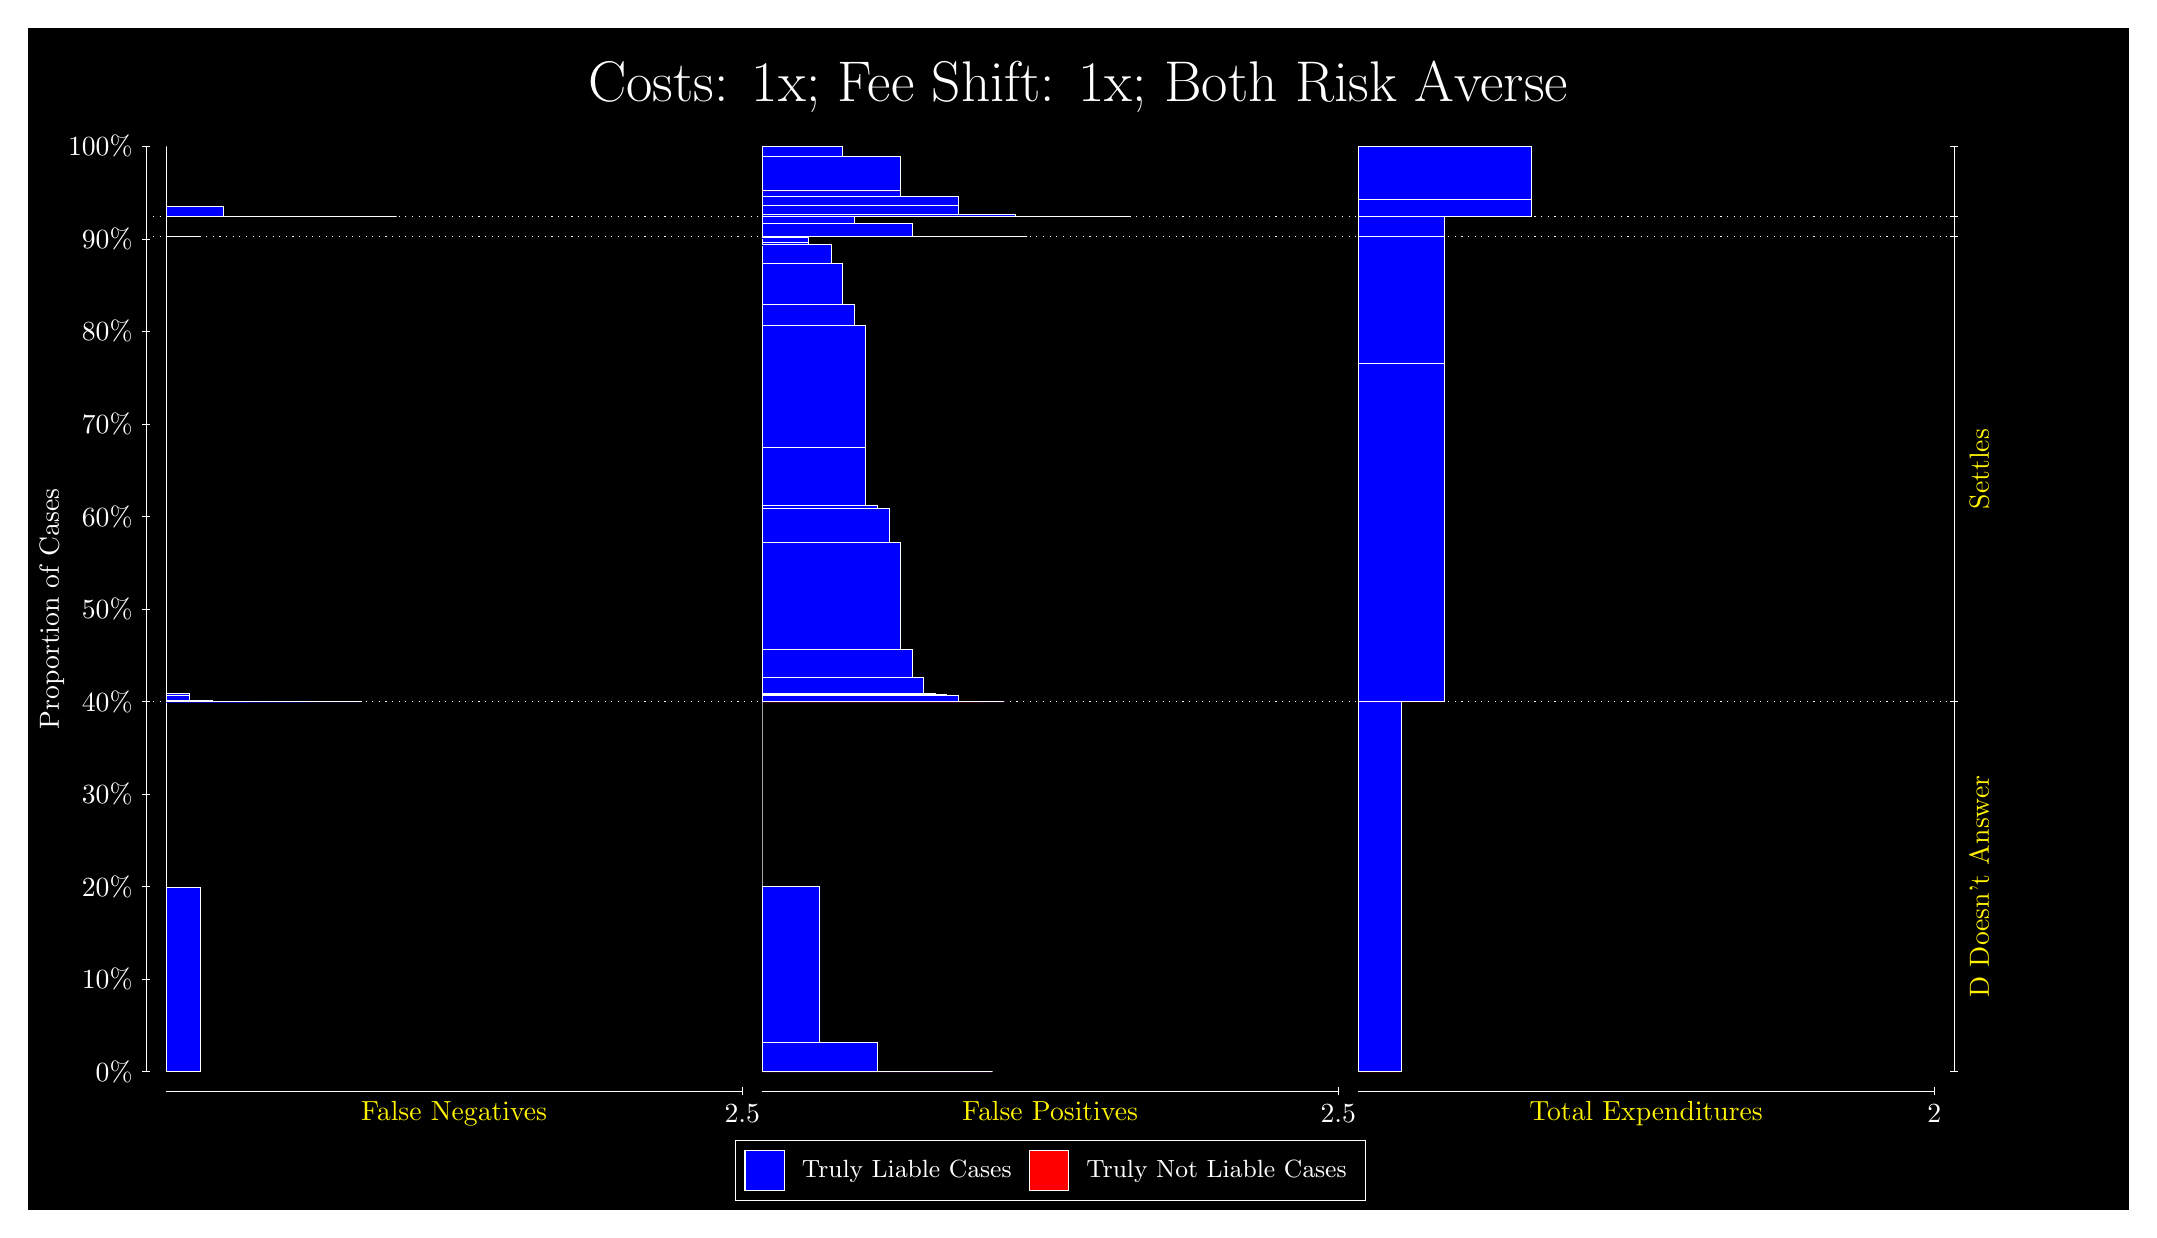
\begin{tikzpicture}
\draw[fill=black] (0,0) rectangle (26.667,15);
\draw[text=white] (0,13.5) rectangle (26.667,15) node[midway] {\huge Costs: 1x; Fee Shift: 1x; Both Risk Averse};
\draw[white, very thin] (1.5,1.75) -- (1.5,13.5);
\node[rotate=90, text=white, anchor=center] at (0.3, 7.625) {Proportion of Cases};
\draw[white, very thin] (1.45,1.75) -- (1.55,1.75);
\node[text=white, anchor=east] at (1.45, 1.75) {0\%};
\draw[white, very thin] (1.45,2.925) -- (1.55,2.925);
\node[text=white, anchor=east] at (1.45, 2.925) {10\%};
\draw[white, very thin] (1.45,4.1) -- (1.55,4.1);
\node[text=white, anchor=east] at (1.45, 4.1) {20\%};
\draw[white, very thin] (1.45,5.275) -- (1.55,5.275);
\node[text=white, anchor=east] at (1.45, 5.275) {30\%};
\draw[white, very thin] (1.45,6.45) -- (1.55,6.45);
\node[text=white, anchor=east] at (1.45, 6.45) {40\%};
\draw[white, very thin] (1.45,7.625) -- (1.55,7.625);
\node[text=white, anchor=east] at (1.45, 7.625) {50\%};
\draw[white, very thin] (1.45,8.8) -- (1.55,8.8);
\node[text=white, anchor=east] at (1.45, 8.8) {60\%};
\draw[white, very thin] (1.45,9.975) -- (1.55,9.975);
\node[text=white, anchor=east] at (1.45, 9.975) {70\%};
\draw[white, very thin] (1.45,11.15) -- (1.55,11.15);
\node[text=white, anchor=east] at (1.45, 11.15) {80\%};
\draw[white, very thin] (1.45,12.325) -- (1.55,12.325);
\node[text=white, anchor=east] at (1.45, 12.325) {90\%};
\draw[white, very thin] (1.45,13.5) -- (1.55,13.5);
\node[text=white, anchor=east] at (1.45, 13.5) {100\%};

\draw[white, very thin] (24.457,1.75) -- (24.457,13.5);
\draw[white, very thin] (24.407,1.75) -- (24.507,1.75);
\node[anchor=west] at (24.407, 1.75) {};
\draw[white, very thin] (24.407,6.4489) -- (24.507,6.4489);
\node[anchor=west] at (24.407, 6.4489) {};
\draw[white, very thin] (24.407,12.355) -- (24.507,12.355);
\node[anchor=west] at (24.407, 12.355) {};
\draw[white, very thin] (24.407,12.609) -- (24.507,12.609);
\node[anchor=west] at (24.407, 12.609) {};
\draw[white, very thin] (24.407,13.5) -- (24.507,13.5);
\node[anchor=west] at (24.407, 13.5) {};

\draw[white, very thin, fill=blue] (1.75,1.75) rectangle (2.1891,4.0962);
\draw[white, very thin, fill=red] (1.75,4.0962) rectangle (1.75,4.0962);
\draw[white, very thin, fill=blue] (1.75,4.0962) rectangle (1.75,6.4489);
\draw[white, very thin, fill=blue] (1.75,6.4489) rectangle (4.2384,6.4489);
\draw[white, very thin, fill=blue] (1.75,6.4489) rectangle (3.6529,6.4489);
\draw[white, very thin, fill=blue] (1.75,6.4489) rectangle (3.5065,6.4489);
\draw[white, very thin, fill=blue] (1.75,6.4489) rectangle (3.3602,6.4489);
\draw[white, very thin, fill=blue] (1.75,6.4489) rectangle (3.0674,6.4489);
\draw[white, very thin, fill=blue] (1.75,6.4489) rectangle (2.921,6.4489);
\draw[white, very thin, fill=blue] (1.75,6.4489) rectangle (2.7746,6.4489);
\draw[white, very thin, fill=blue] (1.75,6.4489) rectangle (2.6283,6.4489);
\draw[white, very thin, fill=blue] (1.75,6.4489) rectangle (2.4819,6.4516);
\draw[white, very thin, fill=blue] (1.75,6.4516) rectangle (2.3355,6.4632);
\draw[white, very thin, fill=blue] (1.75,6.4632) rectangle (2.1891,6.4643);
\draw[white, very thin, fill=blue] (1.75,6.4643) rectangle (2.0428,6.5226);
\draw[white, very thin, fill=blue] (1.75,6.5226) rectangle (2.0428,6.5526);
\draw[white, very thin, fill=blue] (1.75,6.5526) rectangle (1.8964,6.5542);
\draw[white, very thin, fill=red] (1.75,6.5542) rectangle (1.75,6.5542);
\draw[white, very thin, fill=blue] (1.75,6.5542) rectangle (1.75,12.355);
\draw[white, very thin, fill=blue] (1.75,12.355) rectangle (2.1891,12.356);
\draw[white, very thin, fill=red] (1.75,12.356) rectangle (1.75,12.356);
\draw[white, very thin, fill=blue] (1.75,12.356) rectangle (1.75,12.609);
\draw[white, very thin, fill=blue] (1.75,12.609) rectangle (4.6775,12.609);
\draw[white, very thin, fill=blue] (1.75,12.609) rectangle (3.9457,12.609);
\draw[white, very thin, fill=blue] (1.75,12.609) rectangle (3.2138,12.612);
\draw[white, very thin, fill=blue] (1.75,12.612) rectangle (2.4819,12.736);
\draw[white, very thin, fill=red] (1.75,12.736) rectangle (1.75,12.736);
\draw[white, very thin, fill=blue] (1.75,12.736) rectangle (1.75,13.5);
\draw[white, very thin, fill=red] (9.3189,1.75) rectangle (12.246,1.75);
\draw[white, very thin, fill=blue] (9.3189,1.75) rectangle (12.246,1.75);
\draw[white, very thin, fill=blue] (9.3189,1.75) rectangle (11.515,1.7532);
\draw[white, very thin, fill=blue] (9.3189,1.7532) rectangle (10.783,2.126);
\draw[white, very thin, fill=blue] (9.3189,2.126) rectangle (10.051,4.1027);
\draw[white, very thin, fill=blue] (9.3189,4.1027) rectangle (9.3189,6.4489);
\draw[white, very thin, fill=red] (9.3189,6.4489) rectangle (12.393,6.4489);
\draw[white, very thin, fill=blue] (9.3189,6.4489) rectangle (12.393,6.4489);
\draw[white, very thin, fill=red] (9.3189,6.4489) rectangle (12.1,6.4489);
\draw[white, very thin, fill=blue] (9.3189,6.4489) rectangle (12.1,6.4494);
\draw[white, very thin, fill=red] (9.3189,6.4494) rectangle (11.807,6.4494);
\draw[white, very thin, fill=blue] (9.3189,6.4494) rectangle (11.807,6.5322);
\draw[white, very thin, fill=blue] (9.3189,6.5322) rectangle (11.661,6.5454);
\draw[white, very thin, fill=red] (9.3189,6.5454) rectangle (11.515,6.5454);
\draw[white, very thin, fill=blue] (9.3189,6.5454) rectangle (11.515,6.5476);
\draw[white, very thin, fill=blue] (9.3189,6.5476) rectangle (11.368,6.7616);
\draw[white, very thin, fill=red] (9.3189,6.7616) rectangle (11.222,6.7616);
\draw[white, very thin, fill=blue] (9.3189,6.7616) rectangle (11.222,7.1189);
\draw[white, very thin, fill=blue] (9.3189,7.1189) rectangle (11.075,8.4737);
\draw[white, very thin, fill=blue] (9.3189,8.4737) rectangle (10.929,8.8996);
\draw[white, very thin, fill=blue] (9.3189,8.8996) rectangle (10.783,8.9421);
\draw[white, very thin, fill=blue] (9.3189,8.9421) rectangle (10.636,9.683);
\draw[white, very thin, fill=red] (9.3189,9.683) rectangle (10.636,9.683);
\draw[white, very thin, fill=blue] (9.3189,9.683) rectangle (10.636,11.23);
\draw[white, very thin, fill=blue] (9.3189,11.23) rectangle (10.49,11.499);
\draw[white, very thin, fill=blue] (9.3189,11.499) rectangle (10.344,12.01);
\draw[white, very thin, fill=blue] (9.3189,12.01) rectangle (10.197,12.25);
\draw[white, very thin, fill=blue] (9.3189,12.25) rectangle (10.051,12.251);
\draw[white, very thin, fill=blue] (9.3189,12.251) rectangle (9.9044,12.281);
\draw[white, very thin, fill=blue] (9.3189,12.281) rectangle (9.9044,12.34);
\draw[white, very thin, fill=blue] (9.3189,12.34) rectangle (9.758,12.341);
\draw[white, very thin, fill=blue] (9.3189,12.341) rectangle (9.6116,12.352);
\draw[white, very thin, fill=blue] (9.3189,12.352) rectangle (9.4652,12.355);
\draw[white, very thin, fill=blue] (9.3189,12.355) rectangle (9.3189,12.355);
\draw[white, very thin, fill=red] (9.3189,12.355) rectangle (12.686,12.355);
\draw[white, very thin, fill=blue] (9.3189,12.355) rectangle (12.686,12.355);
\draw[white, very thin, fill=blue] (9.3189,12.355) rectangle (11.954,12.36);
\draw[white, very thin, fill=blue] (9.3189,12.36) rectangle (11.222,12.519);
\draw[white, very thin, fill=blue] (9.3189,12.519) rectangle (10.49,12.608);
\draw[white, very thin, fill=blue] (9.3189,12.608) rectangle (9.758,12.609);
\draw[white, very thin, fill=red] (9.3189,12.609) rectangle (14.003,12.609);
\draw[white, very thin, fill=blue] (9.3189,12.609) rectangle (14.003,12.609);
\draw[white, very thin, fill=red] (9.3189,12.609) rectangle (13.271,12.609);
\draw[white, very thin, fill=blue] (9.3189,12.609) rectangle (13.271,12.61);
\draw[white, very thin, fill=red] (9.3189,12.61) rectangle (12.539,12.61);
\draw[white, very thin, fill=blue] (9.3189,12.61) rectangle (12.539,12.632);
\draw[white, very thin, fill=blue] (9.3189,12.632) rectangle (11.807,12.756);
\draw[white, very thin, fill=red] (9.3189,12.756) rectangle (11.807,12.756);
\draw[white, very thin, fill=blue] (9.3189,12.756) rectangle (11.807,12.867);
\draw[white, very thin, fill=blue] (9.3189,12.867) rectangle (11.075,12.937);
\draw[white, very thin, fill=red] (9.3189,12.937) rectangle (11.075,12.937);
\draw[white, very thin, fill=blue] (9.3189,12.937) rectangle (11.075,13.373);
\draw[white, very thin, fill=blue] (9.3189,13.373) rectangle (10.344,13.373);
\draw[white, very thin, fill=blue] (9.3189,13.373) rectangle (10.344,13.497);
\draw[white, very thin, fill=blue] (9.3189,13.497) rectangle (9.6116,13.497);
\draw[white, very thin, fill=blue] (9.3189,13.497) rectangle (9.6116,13.5);
\draw[white, very thin, fill=blue] (9.3189,13.5) rectangle (9.3189,13.5);
\draw[white, very thin, fill=red] (16.888,1.75) rectangle (17.437,1.75);
\draw[white, very thin, fill=blue] (16.888,1.75) rectangle (17.437,6.4489);
\draw[white, very thin, fill=red] (16.888,6.4489) rectangle (17.986,6.4489);
\draw[white, very thin, fill=blue] (16.888,6.4489) rectangle (17.986,10.749);
\draw[white, very thin, fill=red] (16.888,10.749) rectangle (17.986,10.749);
\draw[white, very thin, fill=blue] (16.888,10.749) rectangle (17.986,12.355);
\draw[white, very thin, fill=red] (16.888,12.355) rectangle (17.986,12.355);
\draw[white, very thin, fill=blue] (16.888,12.355) rectangle (17.986,12.609);
\draw[white, very thin, fill=red] (16.888,12.609) rectangle (19.083,12.609);
\draw[white, very thin, fill=blue] (16.888,12.609) rectangle (19.083,12.827);
\draw[white, very thin, fill=red] (16.888,12.827) rectangle (19.083,12.827);
\draw[white, very thin, fill=blue] (16.888,12.827) rectangle (19.083,13.5);
\draw[white, dotted] (1.5,6.4489) -- (24.457,6.4489);
\draw[white, dotted] (1.5,12.355) -- (24.457,12.355);
\draw[white, dotted] (1.5,12.609) -- (24.457,12.609);
\draw[white, very thin] (1.75,1.5) -- (9.0689,1.5);
\node[text=yellow, anchor=north] at (5.4094, 1.5) {False Negatives};
\draw[white, very thin] (9.0689,1.45) -- (9.0689,1.55);
\node[text=white, anchor=north] at (9.0689, 1.45) {2.5};

\draw[white, very thin] (9.3189,1.5) -- (16.638,1.5);
\node[text=yellow, anchor=north] at (12.978, 1.5) {False Positives};
\draw[white, very thin] (16.638,1.45) -- (16.638,1.55);
\node[text=white, anchor=north] at (16.638, 1.45) {2.5};

\draw[white, very thin] (16.888,1.5) -- (24.207,1.5);
\node[text=yellow, anchor=north] at (20.547, 1.5) {Total Expenditures};
\draw[white, very thin] (24.207,1.45) -- (24.207,1.55);
\node[text=white, anchor=north] at (24.207, 1.45) {2};

\node[text=yellow, centered, rotate=90] at (24.777, 4.0994) {D Doesn't Answer};
\node[text=yellow, centered, rotate=90] at (24.777, 9.4019) {Settles};



\draw (12.978300999999998,1.5) node[draw=none] (baseCoordinate) {};
\begin{scope}[align=center]
        \matrix[scale=0.5, draw=white, below=0.5cm of baseCoordinate, nodes={draw}, column sep=0.1cm]{
            \node[rectangle, draw, minimum width=0.5cm, minimum height=0.5cm, fill=blue] {}; &
            \node[draw=none, font=\small, text=white] (B) {Truly Liable Cases}; &
            \node[rectangle, draw, minimum width=0.5cm, minimum height=0.5cm, fill=red] {}; &
            \node[draw=none, font=\small, text=white] (B) {Truly Not Liable Cases}; \\
            };
\end{scope}

\end{tikzpicture}
\end{document}